\chapter{黑洞、吸积盘和 photon ring}
\label{chap:12}

\begin{chapteropening}
黑洞没有可见固体表面，观测到的是它周围物质和光路的结构。吸积盘给出连续谱和随机光变，宽线区把光变延迟转成物理半径，喷流把磁场和相对论运动投影成强偏振，photon ring 把强引力多路径写进长基线可见度和时间延迟。光子事件表中的时间、频率、偏振和干涉相位应尽量保留下来，这些坐标决定了强引力、等离子体和仪器效应能否被分开估计。
\end{chapteropening}

\section{黑洞尺度怎样定下所有坐标}

黑洞问题的自然单位由质量决定：
\begin{equation}
  r_g=\frac{GM}{c^2},\qquad
  t_g=\frac{GM}{c^3},\qquad
  \theta_g=\frac{r_g}{D}.
  \label{eq:ch12-01}
\end{equation}
\begin{formulaexplain}
\(r_g\) 是引力半径，\(t_g\) 是对应光行时，\(\theta_g\) 是角尺度。黑洞质量一旦给定，长度、时间和天空角尺度就都有了共同标尺。
\end{formulaexplain}
这里 \(r_g\) 是引力半径，单位通常用 \(\mathrm{km}\) 或 \(\mathrm{cm}\)；\(t_g\) 是光穿过一个 \(r_g\) 所需的时间；\(D\) 是距离。数值上
\begin{equation}
  r_g=1.477\,{\rm km}\left(\frac{M}{M_\odot}\right),\qquad
  t_g=4.93\,\mu{\rm s}\left(\frac{M}{M_\odot}\right).
  \label{eq:ch12-02}
\end{equation}
\begin{formulaexplain}
这组数值把质量直接换成公里和微秒。它说明同一无量纲吸积过程在 Sgr A* 和 M87* 上会有完全不同的观测时间尺度。
\end{formulaexplain}
Sgr A* 的 \(M\simeq4\times10^6\,M_\odot\)，所以 \(t_g\simeq20\,\mathrm{s}\)，ISCO 量级的变化可以在几分钟内出现。M87* 的 \(M=(6.5\pm0.7)\times10^9\,M_\odot\)，\(t_g\simeq3.2\times10^4\,\mathrm{s}\)，同样的无量纲过程会被拉长到小时到天 \citep{2019ApJ...875L...1E,2019ApJ...875L...6E,2022ApJ...930L..12E}。

黑洞阴影的角直径可以粗略写成
\begin{equation}
  d_{\rm sh}\simeq \kappa\,\theta_g,\qquad \kappa\simeq 10.4 ,
  \label{eq:ch12-03}
\end{equation}
\begin{formulaexplain}
\(d_{\rm sh}\) 是黑洞阴影角直径，\(\kappa\) 是从引力半径到阴影直径的无量纲系数。EHT 测到的环尺度本质上是 \(\theta_g\) 的放大版本。
\end{formulaexplain}
其中 \(\kappa\) 对 Kerr 黑洞的自旋和倾角只有百分之几到十来个百分点的变化。EHT 在 \(1.3\,\mathrm{mm}\) 看到 M87* 的非对称环直径为 \(42\pm3\,\mu{\rm as}\)，中心亮度压低超过十倍；Sgr A* 的厚环直径为 \(51.8\pm2.3\,\mu{\rm as}\)，但源在观测夜内有明显分钟到小时级结构变化 \citep{2019ApJ...875L...4E,2019ApJ...875L...5E,2022ApJ...930L..14E,2022ApJ...930L..15E}。

\begin{figure}[tbp]
\centering
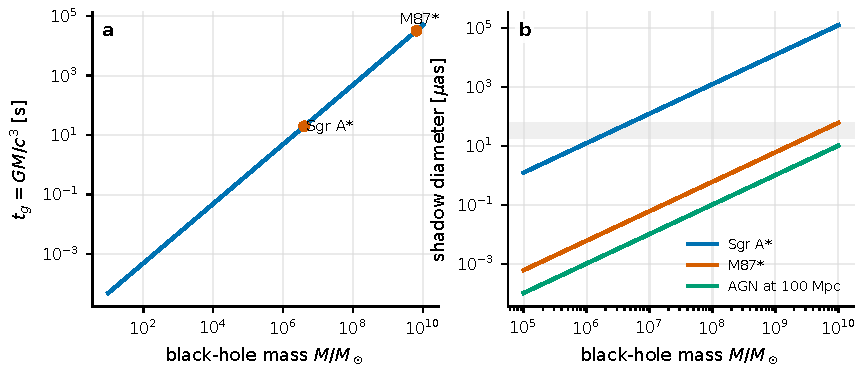
\includegraphics[width=0.94\linewidth]{figures/generated/chapter_12/ch12_black_hole_scales.pdf}
\caption{黑洞时间尺度和角尺度都由质量线性控制。Sgr A* 和 M87* 的质量相差约 \(10^3\)，但距离也相差约 \(10^3\)，所以二者的阴影角直径都在几十微角秒；时间尺度却完全不同，Sgr A* 可以在一次 VLBI 扫描内改变，M87* 的结构更接近静态。}
\label{fig:chapter-12-scales}
\end{figure}

事件表里，黑洞观测的基本坐标扩展为
\[
  (t_i,\nu_i,{\bf b}_i,\eta_i,w_i),
\]
其中 \(t_i\) 是到达时间，\(\nu_i\) 是频率或能道，\({\bf b}_i\) 是投影基线，\(\eta_i\) 是偏振调制角或 Stokes 通道，\(w_i\) 是权重。EHT 的复可见度、GRAVITY 的差分相位、光学监测的光变和偏振巡天都可以看成这张事件表的不同投影。投影前保留时间和偏振，才能比较吸积流变化、喷流扰动和强引力多路径。

\section{吸积盘怎样产生连续谱和随机变异}

标准薄盘把引力势能局部转化为辐射通量：
\begin{equation}
  F(R)=\frac{3GM\dot M}{8\pi R^3}
  \left[1-\left(\frac{R_{\rm in}}{R}\right)^{1/2}\right],
  \label{eq:ch12-04}
\end{equation}
\begin{formulaexplain}
\(F(R)\) 是薄盘单位面积辐射通量，\(\dot M\) 是吸积率，\(R_{\rm in}\) 是内边界。它把引力能释放分配到不同盘半径。
\end{formulaexplain}
其中 \(R\) 是盘半径，\(\dot M\) 是吸积率，\(R_{\rm in}\) 是内边界，常取几倍 \(r_g\) 量级。若盘在局部近似黑体，温度为
\begin{equation}
  T(R)=\left[\frac{F(R)}{\sigma_{\rm SB}}\right]^{1/4}.
  \label{eq:ch12-05}
\end{equation}
\begin{formulaexplain}
\(T(R)\) 是盘的局部有效温度，\(\sigma_{\rm SB}\) 是 Stefan--Boltzmann 常数。薄盘连续谱的颜色来自不同半径黑体温度的叠加。
\end{formulaexplain}
远离内边界时 \(T\propto R^{-3/4}\)，于是某个波长主导的半光半径满足
\begin{equation}
  R_\lambda \propto (M\dot M)^{1/3}\lambda^{4/3}.
  \label{eq:ch12-06}
\end{equation}
\begin{formulaexplain}
\(R_\lambda\) 是波长 \(\lambda\) 附近主要发光的盘半径。波长越长，来自越外层；质量和吸积率越大，盘的同一颜色区域也越大。
\end{formulaexplain}
对 \(M\sim10^8\,M_\odot\)、\(L/L_{\rm Edd}\sim0.1\) 的类星体，光学和近紫外连续谱常来自 \(0.1-10\) light-day 量级的半径。微透镜和多波段延迟经常给出比最简单薄盘更大的光学盘，这就是 inhomogeneous disk 模型和再处理模型被反复讨论的原因 \citep{1973A&A....24..337S,2006ApJ...642...87P,2011ApJ...727L..24D}。

\begin{figure}[tbp]
\centering
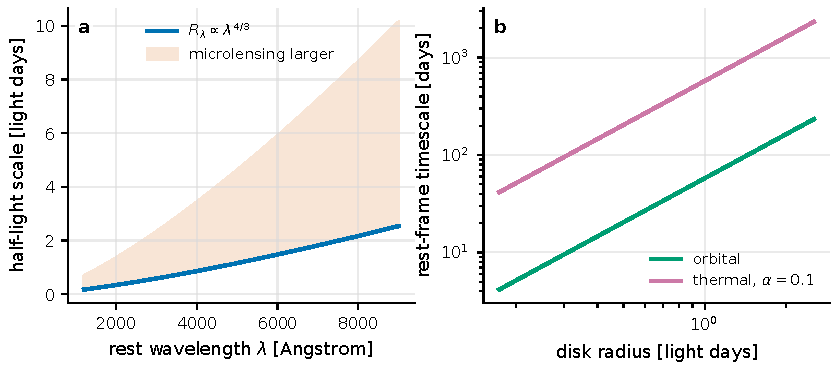
\includegraphics[width=0.94\linewidth]{figures/generated/chapter_12/ch12_accretion_disk_radii.pdf}
\caption{薄盘标度给出 \(R_\lambda\propto\lambda^{4/3}\)。左图的橙色区域表示微透镜和部分连续谱延迟常暗示的更大光学发光面积；右图比较同一半径上的轨道时间和热时间，若 \(\alpha\simeq0.1\)，热时间约为轨道时间的十倍。}
\label{fig:chapter-12-disk}
\end{figure}

盘上一个半径的动力学和热时间分别可估为
\begin{equation}
  t_{\rm orb}=2\pi\left(\frac{R^3}{GM}\right)^{1/2},\qquad
  t_{\rm th}\simeq \frac{t_{\rm orb}}{\alpha}.
  \label{eq:ch12-07}
\end{equation}
\begin{formulaexplain}
\(t_{\rm orb}\) 是 Kepler 轨道时间，\(t_{\rm th}\) 是热时间，\(\alpha\) 是粘滞参数。光变能否快速响应，取决于扰动落在哪个盘时间尺度上。
\end{formulaexplain}
\Needspace{12\baselineskip}
\(\alpha\) 是 Shakura-Sunyaev 粘滞参数，常用 \(0.01-0.3\) 的范围做估计。对 AGN 光学盘，\(t_{\rm orb}\) 可以是几十天到几年，\(t_{\rm th}\) 更长。大样本光学光变常用阻尼随机游走描述：
\begin{equation}
  C(\tau)=\sigma^2\exp\left(-\frac{|\tau|}{\tau_d}\right),
  \qquad
  P(f)\propto\frac{1}{1+(2\pi f\tau_d)^2}.
  \label{eq:ch12-08}
\end{equation}
\begin{formulaexplain}
\(C(\tau)\) 是自协方差，\(P(f)\) 是功率谱，\(\tau_d\) 是阻尼时间。这个模型把随机盘光变写成一个会逐渐失忆的相关过程。
\end{formulaexplain}
这里 \(C(\tau)\) 是光变自协方差，\(\tau_d\) 是阻尼时间，单位通常是 rest-frame day；\(P(f)\) 是功率谱密度。观测上 \(\tau_d\) 和黑洞质量相关，超大质量黑洞常为数十到数百天，白矮星吸积盘也落在相近的质量缩放趋势上 \citep{1993ApJ...406..420M,2021Sci...373..789B,2016Natur.534...75M}。

\begin{figure}[tbp]
\centering
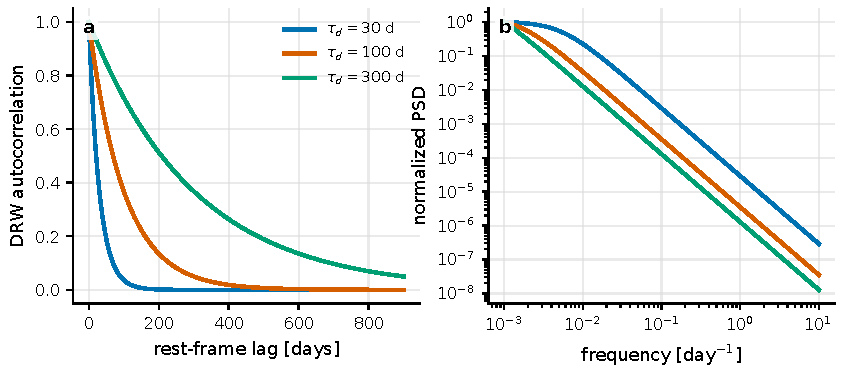
\includegraphics[width=0.94\linewidth]{figures/generated/chapter_12/ch12_variability_autocorrelation.pdf}
\caption{阻尼随机游走模型把随机光变写成一个相关时间。短 \(\tau_d\) 的光变很快失去记忆，功率谱较早转入 \(f^{-2}\) 衰减；长 \(\tau_d\) 的盘在更长时间上保持相关，低频平台延伸得更远。}
\label{fig:chapter-12-variability}
\end{figure}

对光子统计，吸积盘的难点是多模稀释。一个 \(10^8\,M_\odot\) AGN 的光学连续谱来自大量独立湍流区域和多个热时间，单一量子态的 bunching 信号会被空间、频率和时间模式平均掉。可测量的量更可能是相位或颜色条件下的过量相关，例如在一个 flare 前后比较 \(g^{(2)}(\tau)\) 的宽度，或把偏振通道分开看 turbulent cell 的寿命。平均亮度主要给出光子率和归一化；可探测性还受相干时间、采样窗口和经典涨落可建模程度控制。

\section{宽线区怎样把时间延迟和角位移合在一起}

宽线区的传统反响映射写成
\begin{equation}
  L(v,t)=\int \Psi(v,\tau)\,C(t-\tau)\,d\tau ,
  \label{eq:ch12-09}
\end{equation}
\begin{formulaexplain}
\(C(t)\) 是连续谱驱动光变，\(L(v,t)\) 是谱线响应，\(\Psi(v,\tau)\) 是转移函数。BLR 反响映射把时间延迟和速度结构一起编码。
\end{formulaexplain}
其中 \(C(t)\) 是连续谱光变，\(L(v,t)\) 是速度 \(v\) 处的谱线光变，\(\Psi(v,\tau)\) 是转移函数。延迟 \(\tau\) 对应 \(R\simeq c\tau\)，速度宽度给引力势中的轨道速度。经验上 H\(\beta\) 半径和 \(5100\text{\AA}\) 连续谱光度满足
\begin{equation}
  R_{\rm BLR}\simeq 33.7\,{\rm light\,days}
  \left[\frac{\lambda L_\lambda(5100\text{\AA})}{10^{44}\,\mathrm{erg\,s^{-1}}}\right]^{0.533}.
  \label{eq:ch12-10}
\end{equation}
\begin{formulaexplain}
\(R_{\rm BLR}\) 是宽线区半径，\(\lambda L_\lambda\) 是 \(5100\text{\AA}\) 连续谱光度。这个经验关系让单历元光谱也能估计 BLR 尺度。
\end{formulaexplain}
这个关系的散布来自宿主星光扣除、采样窗口、各向异性照明、线种差异和 BLR 几何差异。黑洞质量常写为
\begin{equation}
  M_{\rm BH}=f_{\rm vir}\frac{R_{\rm BLR}\Delta V^2}{G},
  \label{eq:ch12-11}
\end{equation}
\begin{formulaexplain}
\(M_{\rm BH}\) 是黑洞质量，\(\Delta V\) 是宽线速度宽度，\(f_{\rm vir}\) 是几何因子。它是用 BLR 半径和轨道速度做的 virial 质量估计。
\end{formulaexplain}
其中 \(\Delta V\) 是谱线宽度，\(f_{\rm vir}\) 吸收倾角和速度场几何。对 Seyfert，\(\tau\) 可以是几天到几十天；对亮类星体，\(\tau\) 可达数百天，监测窗口和季节间断会成为主要系统误差 \citep{1982ApJ...255..419B,1993PASP..105..247P,2013ApJ...767..149B}。

干涉相位给 BLR 另一种投影。若谱线某个速度通道的光心相对连续谱偏移 \(\boldsymbol{\delta\theta}(v)\)，基线 \({\bf B}\) 上的差分相位近似为
\begin{equation}
  \Delta\varphi(v)\simeq
  2\pi\frac{{\bf B}\cdot\boldsymbol{\delta\theta}(v)}{\lambda}.
  \label{eq:ch12-12}
\end{equation}
\begin{formulaexplain}
\(\Delta\varphi(v)\) 是速度通道的差分相位，\({\bf B}\) 是基线，\(\boldsymbol{\delta\theta}\) 是光心偏移。相位直接测的是谱线发光区的角位移投影。
\end{formulaexplain}
这里 \(\Delta\varphi\) 用弧度，\({\bf B}\) 用米，\(\lambda\) 用米，\(\boldsymbol{\delta\theta}\) 用弧度。GRAVITY 对 3C 273 的 Pa\(\alpha\) 谱线测到红蓝翼光心沿近似垂直喷流方向的梯度，模型给 \(R_{\rm BLR}=46\pm10\,\mu{\rm as}\)，对应约 \(145\) light-days，并得到接近 face-on 的厚盘旋转几何 \citep{2018Natur.563..657G}。

\begin{figure}[tbp]
\centering
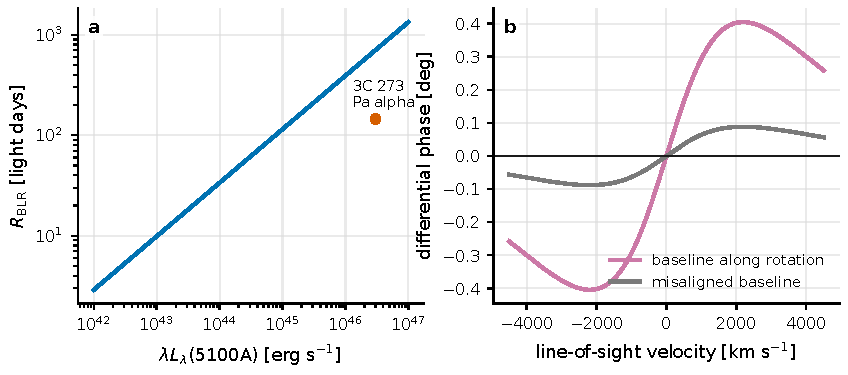
\includegraphics[width=0.94\linewidth]{figures/generated/chapter_12/ch12_blr_reverberation_interferometry.pdf}
\caption{BLR 的时间和角度信息互补。左图是 H\(\beta\) 半径-光度关系，时间延迟给物理半径；右图示意旋转 BLR 的红蓝翼会在基线上产生反号差分相位，基线若与旋转轴几何不匹配，相位振幅会被压低。}
\label{fig:chapter-12-blr}
\end{figure}

强度干涉若用于谱线区，测到的是窄带角结构的 \(|V|^2\)，与 GRAVITY 的差分相位不同。它更适合亮、低红移、宽线强、角尺度大的目标。设 BLR 半径 \(R_{\rm BLR}=100\) light-days，角直径为
\begin{equation}
  \theta_{\rm BLR}\simeq 2\frac{R_{\rm BLR}}{D_A}
  \simeq 11\,\mu{\rm as}
  \left(\frac{R_{\rm BLR}}{100\,{\rm light\,days}}\right)
  \left(\frac{100\,{\rm Mpc}}{D_A}\right),
  \label{eq:ch12-13}
\end{equation}
\begin{formulaexplain}
\(\theta_{\rm BLR}\) 是 BLR 角直径，\(D_A\) 是角直径距离。若时间延迟给物理半径、干涉给角半径，就能形成几何距离。
\end{formulaexplain}
这已经要求百米到公里级基线和非常高的光子通量。若同时有反响映射给 \(R_{\rm BLR}\) 和干涉给 \(\theta_{\rm BLR}\)，可以形成几何距离 \(D_A=2R_{\rm BLR}/\theta_{\rm BLR}\)，但误差会被倾角、BLR 各向异性、线区厚度和宿主污染放大。

\section{喷流偏振怎样把磁场几何带进光子统计}

旋转黑洞和磁通量可以给喷流供能。Blandford-Znajek 机制的常用标度是
\begin{equation}
  P_{\rm BZ}\sim \frac{\kappa}{4\pi c}\Phi_{\rm BH}^2\Omega_H^2,
  \label{eq:ch12-14}
\end{equation}
\begin{formulaexplain}
\(P_{\rm BZ}\) 是 Blandford--Znajek 喷流功率标度，\(\Phi_{\rm BH}\) 是黑洞磁通量，\(\Omega_H\) 是视界角速度。自旋和磁通量共同决定可抽取功率。
\end{formulaexplain}
其中 \(\Phi_{\rm BH}\) 是穿过黑洞的磁通量，\(\Omega_H\) 是视界角速度，\(\kappa\) 是与场结构有关的无量纲系数。对 M87* 这类低吸积率射电星系，EHT 偏振显示视界尺度附近存在有序磁场，和磁控吸积流及喷流功率的图像相容 \citep{1977MNRAS.179..433B,1979ApJ...232...34B,2021ApJ...910L..13E}。

喷流光学和近红外通常来自同步辐射。电子 Lorentz 因子 \(\gamma_e\) 在磁场 \(B\) 中的特征频率为
\begin{equation}
  \nu_{\rm syn}\simeq
  4.2\times10^6\,{\rm Hz}\,
  \frac{\delta}{1+z}
  \left(\frac{B}{1\,{\rm G}}\right)\gamma_e^2 ,
  \label{eq:ch12-15}
\end{equation}
\begin{formulaexplain}
\(\nu_{\rm syn}\) 是同步辐射特征频率，\(B\) 是磁场，\(\gamma_e\) 是电子 Lorentz 因子，\(\delta\) 是 Doppler 因子。它把观测频率换成喷流电子能量。
\end{formulaexplain}
其中 \(\delta\) 是 Doppler 因子，\(z\) 是红移。若 \(B\simeq0.1-1\,\mathrm{G}\)、\(\delta\simeq10\)，光学 \(\nu\sim5\times10^{14}\,\mathrm{Hz}\) 需要 \(\gamma_e\sim10^4\)。幂律电子 \(N(E)\propto E^{-p}\) 的最大线偏振度为
\begin{equation}
  \Pi_{\rm max}=\frac{p+1}{p+7/3},
  \label{eq:ch12-16}
\end{equation}
\begin{formulaexplain}
\(\Pi_{\rm max}\) 是理想同步辐射最大线偏振度，\(p\) 是电子能谱指数。实际偏振低于它，通常说明有多个磁场方向在视线内相加。
\end{formulaexplain}
对 \(p=2-3\)，\(\Pi_{\rm max}\simeq70\%-75\%\)。真实 blazar 通常只有几百分比到几十百分比，因为多个磁场胞元、冲击、剪切和湍流会把 Stokes 向量相加抵消。跨频触发时，光学偏振角旋转、\(\gamma\) 射线 flare 和射电 knot 抛射若时间相符，通常指向同一个喷流扰动穿过不同发光区 \citep{1995PASP..107..803U,2008Natur.452..966M}。

偏振分辨的二阶相关可以写成
\begin{equation}
  g^{(2)}_{QU}(\tau)=
  \frac{\langle \delta Q(t)\delta U(t+\tau)\rangle}
  {\sigma_Q\sigma_U},
  \label{eq:ch12-17}
\end{equation}
\begin{formulaexplain}
\(g^{(2)}_{QU}(\tau)\) 是两个 Stokes 涨落之间的归一化相关。它把喷流磁场方向变化写成可随延迟 \(\tau\) 测量的偏振统计。
\end{formulaexplain}
这个量描述磁场方向的随机过程在两个 Stokes 分量之间如何延迟。若 shock-in-jet 模型正确，\(Q,U\) 的相关时间应接近扰动穿过光学发光区的时间；若湍流胞元主导，相关函数会更快衰减，且在不同颜色上不完全同步。

\section{Photon ring 怎样进入图像、可见度和时间结构}

干涉仪测的是天空亮度的 Fourier 分量：
\begin{equation}
  V({\bf u})=\int I({\boldsymbol\theta})
  e^{-2\pi i{\bf u}\cdot{\boldsymbol\theta}}\,d^2\theta,
  \qquad {\bf u}=\frac{{\bf B}_\perp}{\lambda}.
  \label{eq:ch12-18}
\end{equation}
\begin{formulaexplain}
\(V({\bf u})\) 是复可见度，\(I({\boldsymbol\theta})\) 是天空亮度，\({\bf u}\) 是以波长为单位的投影基线。干涉仪测的是天空图像的 Fourier 分量。
\end{formulaexplain}
一个均匀薄环的可见度近似为
\begin{equation}
  V(u)\simeq J_0(\pi d u),
  \label{eq:ch12-19}
\end{equation}
\begin{formulaexplain}
\(J_0\) 是零阶 Bessel 函数，\(d\) 是环直径，\(u\) 是基线长度对应的空间频率。薄环会在可见度中产生振荡和零点。
\end{formulaexplain}
其中 \(d\) 是环直径，单位弧度。M87* 的 \(d\simeq42\,\mu{\rm as}\)，所以 Earth-size \(1.3\,\mathrm{mm}\) VLBI 已经能看到第一个可见度谷和环状结构。若环有有限宽度 \(w\)，长基线振荡会被包络压低；宽吸积流比窄 photon ring 更快被解析掉 \citep{2019ApJ...875L...2E,2019ApJ...875L...3E,2020SciA....6.1310J}。

\begin{figure}[tbp]
\centering
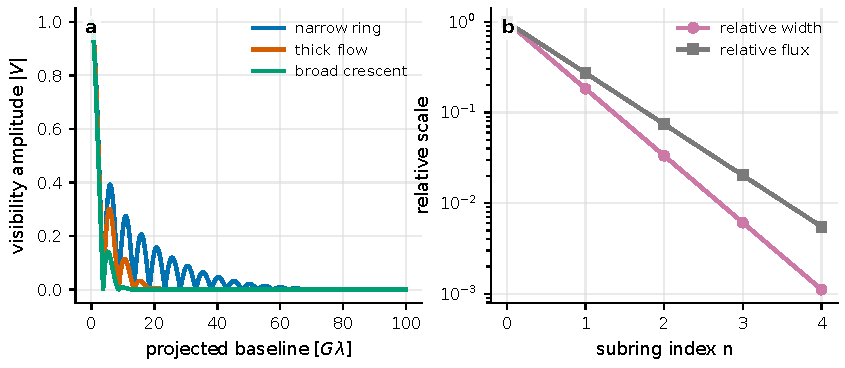
\includegraphics[width=0.94\linewidth]{figures/generated/chapter_12/ch12_photon_ring_visibility.pdf}
\caption{环状结构在长基线可见度中产生振荡。左图比较同样 \(42\,\mu{\rm as}\) 直径下不同厚度的环，窄环在更长基线上仍保留振荡；右图示意 photon subring 的宽度和通量随环绕次数下降，高阶子环通量小，但在足够长的基线可留下普适结构。}
\label{fig:chapter-12-photon-ring}
\end{figure}

EHT 图像中的亮环包含直接图像、一次透镜图像和高阶 photon subring，并不是数学上无限薄的 photon ring。吸积流厚度、光深、湍流和时间平均会把强引力的窄结构涂宽。Gralla 等强调，高阶 photon ring 在总通量中常很小；Johnson 等指出，足够长基线会解析掉宽的吸积流，只留下窄子环的普适振荡。可以把第 \(n\) 个子环的宽度和通量写成标度形式
\begin{equation}
  w_n\simeq w_0 e^{-\gamma n},\qquad
  F_n\simeq F_0 e^{-\beta n},
  \label{eq:ch12-20}
\end{equation}
\begin{formulaexplain}
\(w_n\) 和 \(F_n\) 是第 \(n\) 个 photon subring 的宽度和通量。指数标度描述多圈光路逐层变窄、变暗的强引力结构。
\end{formulaexplain}
其中 \(\gamma\) 与 photon orbit 的 Lyapunov 指数有关，\(\beta\) 还取决于发射和吸收。这个标度刻画强引力多圈光路的指数嵌套角结构；实际观测还要接上发射、吸收和时间平均模型 \citep{2019PhRvD.100b4018G,2020PhRvD.102l4004G,2013ApJ...777..170J}。

\Needspace{12\baselineskip}
多路径还意味着时间结构。若第 \(n\) 圈和第 \(n+1\) 圈光路的平均延迟差近似为 photon orbit 周期 \(T_\gamma\)，则相关函数中可能出现
\begin{equation}
  C(\tau)=\langle \delta I(t)\delta I(t+\tau)\rangle
  \quad\hbox{在}\quad
  \tau\simeq mT_\gamma
  \label{eq:ch12-21}
\end{equation}
\begin{formulaexplain}
\(C(\tau)\) 是强度自相关，\(T_\gamma\) 是 photon orbit 周期，\(m\) 是整数。若多路径贡献可见，相关函数可能在这些延迟附近出现弱峰。
\end{formulaexplain}
附近的弱峰。对 Sgr A*，\(T_\gamma\) 是分钟量级，和吸积流本身的 flare 时间重叠；对 M87*，它是天量级，源更稳定但观测调度更难。要把这类峰解释成强引力多路径，需要同时排除喷流 shock、盘湍流、散射屏、采样窗口和校准误差。偏振版本还可比较 \(Q,U,V\) 的延迟结构，EHT 对 M87* 和 Sgr A* 的偏振成像已经展示了这种信息的价值 \citep{2020PhRvD.101h4020H,2021PhRvD.104d4049G,2022PhRvD.106d3021C}。

\section{Hawking 温度为什么不是近期观测主线}

前几节讨论的是普通辐射如何被黑洞附近的强引力、等离子体和磁场组织。真正属于黑洞本身的量子辐射要从一个完全不同的数量级开始：Hawking 温度为
\begin{equation}
  T_H=\frac{\hbar c^3}{8\pi G M k_B}
  \simeq 6.17\times10^{-8}\,{\rm K}
  \left(\frac{M_\odot}{M}\right).
  \label{eq:ch12-22}
\end{equation}
\begin{formulaexplain}
\(T_H\) 是 Hawking 温度，和黑洞质量 \(M\) 成反比。天体质量黑洞温度极低，所以不会成为近期普通望远镜观测主线。
\end{formulaexplain}
恒星质量黑洞的 \(T_H\) 已经远低于 \(2.725\,\mathrm{K}\) 的 CMB；Sgr A* 和 M87* 更低到 \(10^{-14}-10^{-17}\,\mathrm{K}\)。蒸发时间近似为
\begin{equation}
  t_{\rm evap}\simeq
  2.1\times10^{67}\,{\rm yr}
  \left(\frac{M}{M_\odot}\right)^3 .
  \label{eq:ch12-23}
\end{equation}
\begin{formulaexplain}
\(t_{\rm evap}\) 是 Hawking 蒸发时间，随 \(M^3\) 增长。恒星质量和超大质量黑洞的蒸发时间远超宇宙年龄。
\end{formulaexplain}
普通天体黑洞的 Hawking 辐射远低于可预见望远镜灵敏度。只有假设很轻的原初黑洞，温度才会上升到高能波段；这类约束属于宇宙学和高能瞬变。对恒星质量和超大质量黑洞，近期观测主线仍是吸积流、偏振、可见度和 photon ring \citep{1974Natur.248...30H,1975CMaPh..43..199H}。

\begin{figure}[tbp]
\centering
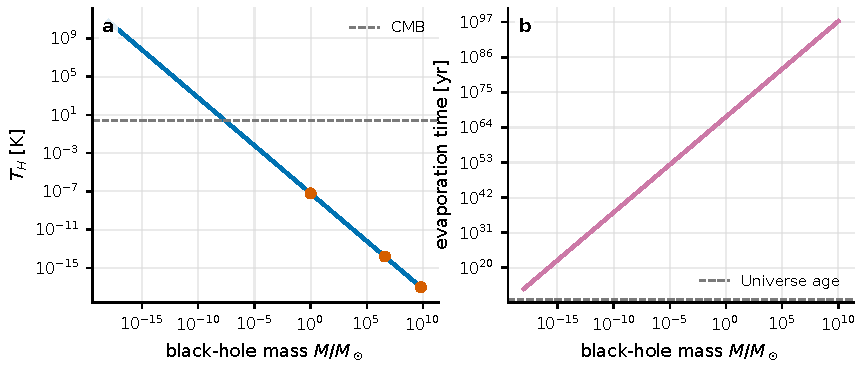
\includegraphics[width=0.94\linewidth]{figures/generated/chapter_12/ch12_hawking_temperature_scale.pdf}
\caption{Hawking 温度随质量反比下降，蒸发时间随质量三次方增加。恒星质量和超大质量黑洞的温度远低于 CMB，蒸发时间远超宇宙年龄；近期可操作的黑洞观测主要来自吸积流、偏振、可见度和时间结构。}
\label{fig:chapter-12-hawking}
\end{figure}

